%!TEX root = main.tex


In this section, we describe in detail a two-phase workflow that makes use of
human computation, natural language processing techniques, and statistical
machine learning methods to cluster complex information. Our method works with
datasets containing 75 to 100 short web clips that answer specific questions
(e.g.,``What does a planet need to support life?'' or ``How do I unclog my
bathtub drain?''). As described in the Experimental Settings Section,
the dataset is gathered by hiring crowdworkers to forage information from the
Web that answers questions from a wide variety of domains. Like most Web
datasets, the datasets we use also contain 10\% to 31\% of clips that contains
little or no useful information for answering the questions. An overview of the
proposed workflow is shown in Figure~\ref{fig:workflow}.

\begin{figure*}[!t]
	\centering
	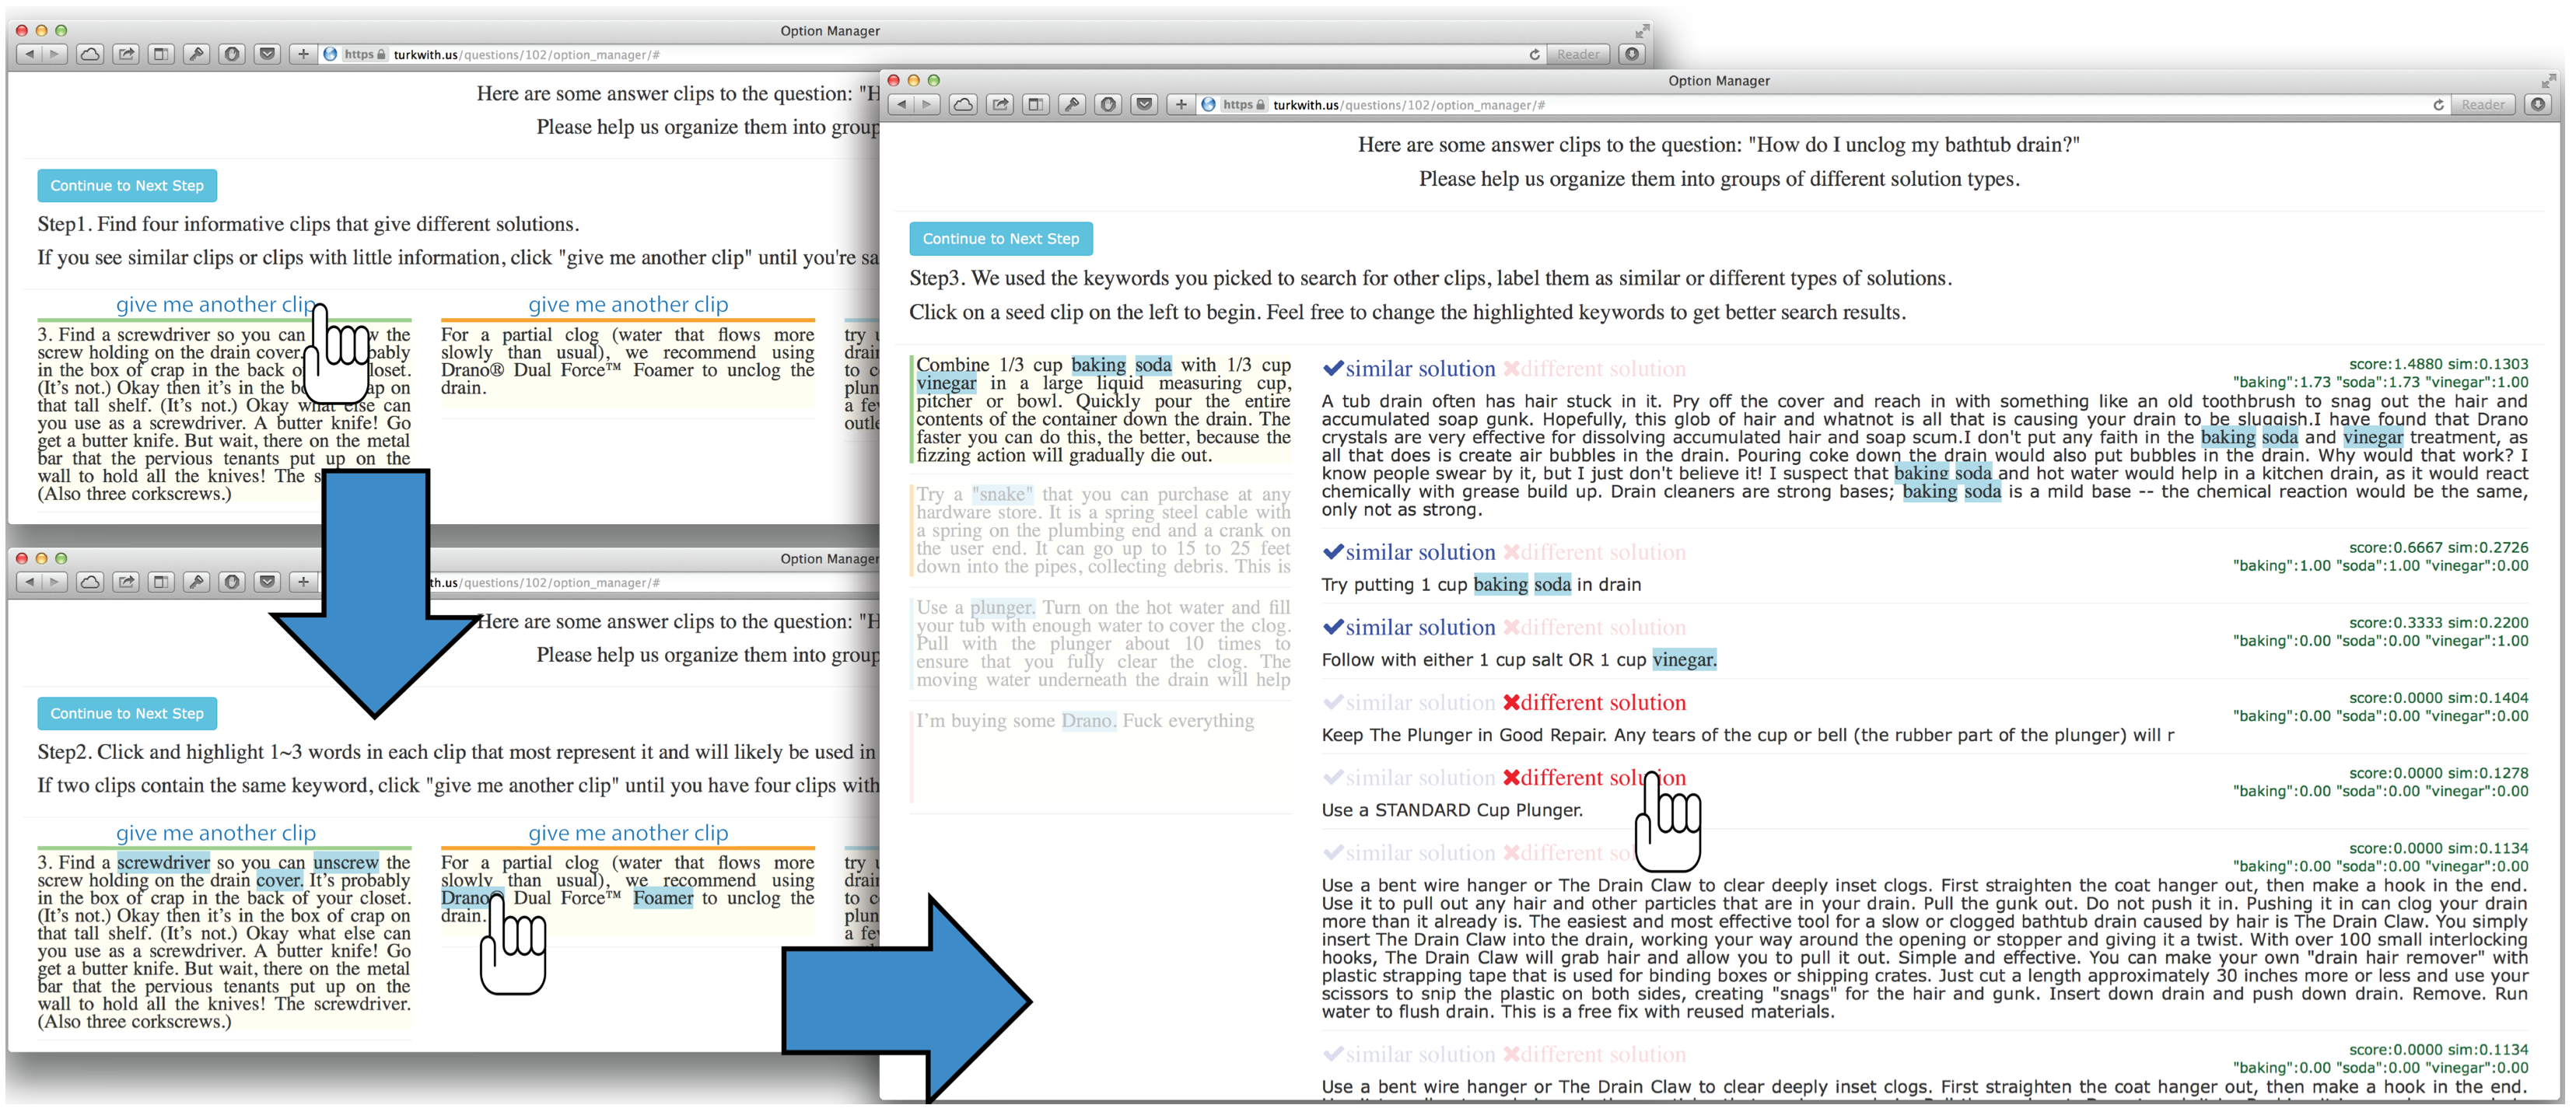
\includegraphics[width=2.1\columnwidth]{images/raw-02.png}
	\caption{The three steps HIT for Phase A: 1. Seed selection, 2. Keyword
		highlighting, and 3. Partial clustering.}
	\label{fig:phase1-hit}
\end{figure*}

\subsection{Hierarchical Clustering}
\label{sec:hclustering}
Before presenting the main process, we first describe a general hierarchical
clustering process that is used throughout the proposed method, and also in the
baseline systems.

Given a similarity metric between any two clips in the dataset and a stopping
threshold, the hierarchical clustering method initially treats each clip as 
a cluster by itself, and iteratively merges the two most similar clusters until a
similarity threshold is reached. After that, each singleton cluster is merged with
the most similar non-singleton cluster (classification). The similarity
between two clusters is defined as:

\begin{equation}
	ClusterSim(\omega_1, \omega_2) = \frac{1}{|\omega_1||\omega_2|} \sum_j \sum_k ClipSim(t_j, t_k)
\end{equation}

where $\omega_1$ and $\omega_2$ are the two clusters, $t_j$ and $t_k$ are each of the
clips in $\omega_1$ and $\omega_2$, respectively, and the $ClipSim()$ function is
the given similarity function between any two clips in the dataset.


\subsection{Phase A: Partial Clustering}

The intuition behind the first part of the system is that a few
keywords can potentially help identify important clusters that covers a
large portion of the dataset \cite{huang2006text}. However, identifying such
salient words often requires in-depth understanding of the textual data.

The goal of Phase A is to make use of human computation to identify a set of
keyword features and train an SVM model to partially cluster the given
dataset.  Since it is infeasible to ask a crowdworker to organize the entire
collection of short texts due to its size, each crowdworker
worked on a small part of the dataset.  We designed an interactive interface
that lets crowdworkers focus on creating four clusters by randomly sampling
the dataset.  The output of this phase is an incomplete set of clusters
and some unclustered clips.  The work in Phase A consists of three stages: First,
partially cluster the given dataset and identify important keywords using the
crowd (Stage 1), Then, train an SVM model to predict pairwise similarity of items in
the dataset (Stage 2). Finally, create clusters using the hierarchical clustering
method (Stage 3). We now describe each stage in turn.

\begin{figure}
\footnotesize
\hrule
\vspace{2 pt}
\textbf{Input:}\\
\indent \ \ \ \ \ \ \ $T$: \ Dataset of Web clips\\
\indent \ \ \ \ \ \ \ $R$: \ A random sample of 4 clips $\{r_1 \sim r_4\} \subset T$ \\
\indent \ \ \ \ \ \ \ $w_i$: \ The ith crowdworker\\
%\vspace{2mm}
\textbf{Output:} \\
\indent \ \ \ \ \ \ \ $S_{i,j}$: \ A subset of $T$ similar to to $r_{i,j} \in R$\\
\indent \ \ \ \ \ \ \ $K_{i,j}$: \ A set of keywords in $r_{i,j}$ \\
\textbf{Description:}
\begin{algorithmic}[1]
\STATE \textbf{For} each crowdworker $w_i$:
   \STATE \ \ \  Sample $R$ from $T$ and present to $w_i$
   \STATE \ \ \  Instruct $w_i$ to replace clips in $R$ by resampling $T$
   \STATE \ \ \  Instruct $w_i$ to highlight keywords $K_{i,j} \subset r_{i,j} \in R$
   \STATE \ \ \  Store each $\{r_{i,j}, K_{i,j}\}$ as $Seed_{i,j}$
\vspace{1mm}
\STATE \ \ \ \textbf{For} each $r_{i,j}, K_{i,j}$ in $Seed_{i,j}$:
   \STATE  \ \ \ \ \ \ Search $T$ using $r_{i,j}, K_{i,j}$ as $S_{i,j}$
   \STATE  \ \ \ \ \ \ Instruct $w_i$ to label each clip in $S_{i,j}$ \\
   \ \ \ \ \ \ \ \ \ \ \ \ \ \ \ \ \ \ \ \ \ \ \ \ \ \ as "similar" or "different"
\STATE \textbf{Return} each $S_{i,j}$ and $K_{i,j}$
\end{algorithmic}
\hrule
\label{fig:phaseAstage1}
\caption{Pseudocode for Phase A: Stage 1}
\end{figure}


\subsubsection{Stage 1. Partial clustering and keyword extraction}

In the first stage of Phase A, we instruct each crowdworker to process a
portion of the input dataset by randomly drawing four seed clips, and searching
the entire corpus by highlighting keywords.  As shown in
Figure~\ref{fig:phase1-hit} , the Human Intelligence Task (HIT) for Stage 1
consists of three steps:

\begin{enumerate}
	\item Four random seed clips are presented to each crowdworker. Above each
		clip, there is a button for replacing the clip with another random clip
		from the corpus.  The crowdworker is then asked to
		replace any clip that either contains little useful information (noise) or is
		too similar to the other seed clips. The workers repeatedly replaces clips
		until they are satisfied with the four clips at hand. Context is
		provided by presenting the initial question for the dataset,
		and multiple items being considered in the dataset.
	\item Crowdworker is then instructed to highlight between one and three
		unique keywords from each of the four seed clips that best describe
		their topics.  At this point, they can still replace any seed clips at
		will, if they find clips that are redundant (containing overlapping
		keywords). This highlighting process further ensures that the workers
		understand the seed clips they have chosen.
	\item For each of the four seed clips, we then automatically search for
		similar clips from the entire corpus based on TF-IDF cosine similarity
		between the clips and the highlighted keywords. The crowdworker is
		asked to label the top 9 search results as \emph{similar} to or
		\emph{different} from their seed clips.
\end{enumerate}

The output of this stage is a number of potentially overlapping clusters, each
contain one seed clip and nine other clips labeled as ``similar'' or
``different''.

% unclear
%\begin{figure}[!h]
%	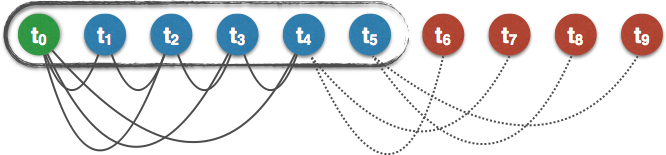
\includegraphics[width=0.9\columnwidth]{images/svm-clusters.png}
%	\caption{In Phase1 Stage1, crowdworkers create a cluster by selecting a
%		seed clip (green), and labeling 9 other clips as similar (blue) or
%		different (red). Each line connecting two clips indicates a training
%		events for Stage2.}
%	\label{fig:svm-clusters}
%\end{figure}

In Figure \ref{fig:phase1-example}, we show two example clips from the datasets
collected using the two questions: ``How do I get my tomato plants to produce
more tomatoes?'' and ``What does a planet need to support life?''
The highlighted words in each clips are the keywords selected by
one of the crowdworkers.

\begin{figure}[!h]
	\fbox{ \vbox{

		\ttfamily
		\small

% bad example
%		We had that problem too.  We snaked the bathroom tub, sink, \& stool so
%		many times.  The answer came to us when we had to replace the stool.
%		We found a \hilight{plumber} in the \hilight{yellow} \hilight{pages}.
%		Got some good recommendations.  They came and snaked the stack!  You
%		have to go on the roof for that.  If you can access the stack, rent as
%		big a plumber's snake as possible and to the job yourself.  Be sure to
%		ask the rental agency lots of questions, they want their equipment back
%		in good shape too. Be sure to clean the snaket (sic) off too.  That is
%		just plain common courtesy.  You will save lots of little tub snaking
%		jobs in the future
%
%		\rule{\columnwidth}{0.4pt}

		Tomato seedlings will need either strong, direct \hilight{sunlight} or
		14-18 hours under grow \hilight{lights}. Place the young plants only a
		couple of inches from florescent grow lights. Plant your tomatoes
		outside in the sunniest part of your vegetable plot.

		\rule{\columnwidth}{0.4pt}

		An absolute requirement for life is an energy source, and the notion of
		planetary habitability implies that many other geophysical,
		geochemical, and astrophysical criteria must be met before an
		astronomical body can support life. In its astrobiology roadmap, NASA
		has defined the principal habitability criteria as "extended regions of
		\hilight{liquid} \hilight{water}, conditions favourable for the
		assembly of complex organic molecules, and energy sources to sustain
		metabolism

	}}
	\caption{Example clips from two different datasets with keywords
		highlighted by crowdworkers.}
	\label{fig:phase1-example}
\end{figure}


\begin{figure}
\footnotesize
\hrule
\vspace{2 pt}
\textbf{Input:}\\
\indent \ \ \ \ \ \ \ $S_{i,j}$: \ Sets of similar and different clips from Phase A Stage 1\\
\indent \ \ \ \ \ \ \ $K$: The set of all keywords from Phase A Stage 1 \\
\textbf{Output:} \\
\indent \ \ \ \ \ \ \ \textit{Clusters}: Clusters of similar clips \\
\indent \ \ \ \ \ \ \ \textit{Singletons}: Unclustered clips \\
\textbf{Description:}
\begin{algorithmic}[1]
\STATE Let \textit{Sim} = \{$(t, t')$ $t, t' \in S_{i,j}$, $t, t'$ labaled "Similar"\}
\STATE Let \textit{Diff} = \{$(t, t')$ $t$ labaled "Similar", $t'$ labaled "Different"\}
\STATE \textbf{For} each $event_i \in$ \textit{Sim} $\cup$ \textit{Diff}:
    \STATE \ \ \ \ \ \ Let $label_i$ = \textit{yes}, if $event_i \in$ \textit{Sim}, \textit{no} otherwise \\
    \STATE \ \ \ \ \ \ Generate feature $feat_{i}$ based on $t, t', K$
\STATE Train classifier \textit{M} using $label$, and $feat$
\STATE \textit{Clusters}, \textit{Singletons} = HierchicalCluster($D$, $M$)
\STATE \textbf{Return} \textit{Clusters}, \textit{Singletons}
\end{algorithmic}
\hrule
\label{fig:phaseAstage2stage3}
\caption{Pseudocode for Phase A: Stages 2 and 3}
\end{figure}

\subsubsection{Stage 2. Distance function: training a SVM model}

In the second stage of Phase A, we use labels and keywords created by
crowdworkers in Stage 1 to train an SVM model in real-time to predict whether a
pair of clips in the dataset belong to the same cluster. The training events
are all possible pairwise combinations of clips in the clusters from Stage 1,
which may include both positive (similar) and negative (different) training
events.  The feature dimensions are all the keywords highlighted by the
crowdworkers in Stage 1, where the value of each dimension is the product of
the number of times that keyword occurred in the two clips.

In general,  the keywords labeled by the crowdworkers contain little irrelevant information
compared to all words in the clips, but there could
still be some highlighted words that are not indicative of a category. For
example, one crowdworker worked on the dataset for ``\emph{How do I unclog my
	bathtub drain?}'' labeled ``\emph{use}'', ``\emph{a}'', and ``\emph{plunger}'' as
the three keywords for a seed clip. Even though \emph{plunger} is a very
indicative feature for clustering this dataset, the first two highlighted words
seem too general to be useful. This can potentially be solved by allowing turkers to extract
bi-gram or tri-gram features from the clips, but it will also increase interface
complexity and decrease the coverage of the identified features (e.g.,
\emph{plunger} versus \emph{use a plunger}). On the other hand, a linear
Support Vector Machine analyzes all training events using a linear kernel to
assign weights to different dimensions (i.e., keywords), which seems well suited for
our purpose \cite{chang2011libsvm, wu2004probability}.

\subsubsection{Stage 3. Hierarchical clustering}

In the third and final stage of Phase A, we use the SVM model trained in the
previous stage to predict whether two clips belong to the same cluster. With
the probability output of the SVM model as the similarity function between
clips, and a threshold of 0.5 probability, we perform the hierarchical
clustering as described in the previous subsection.  However, we do not merge
singleton clusters with non-singleton clusters at this stage, so the output of
this stage is a set of clusters and unclustered clips.

\begin{figure*}[!t]
	\centering
	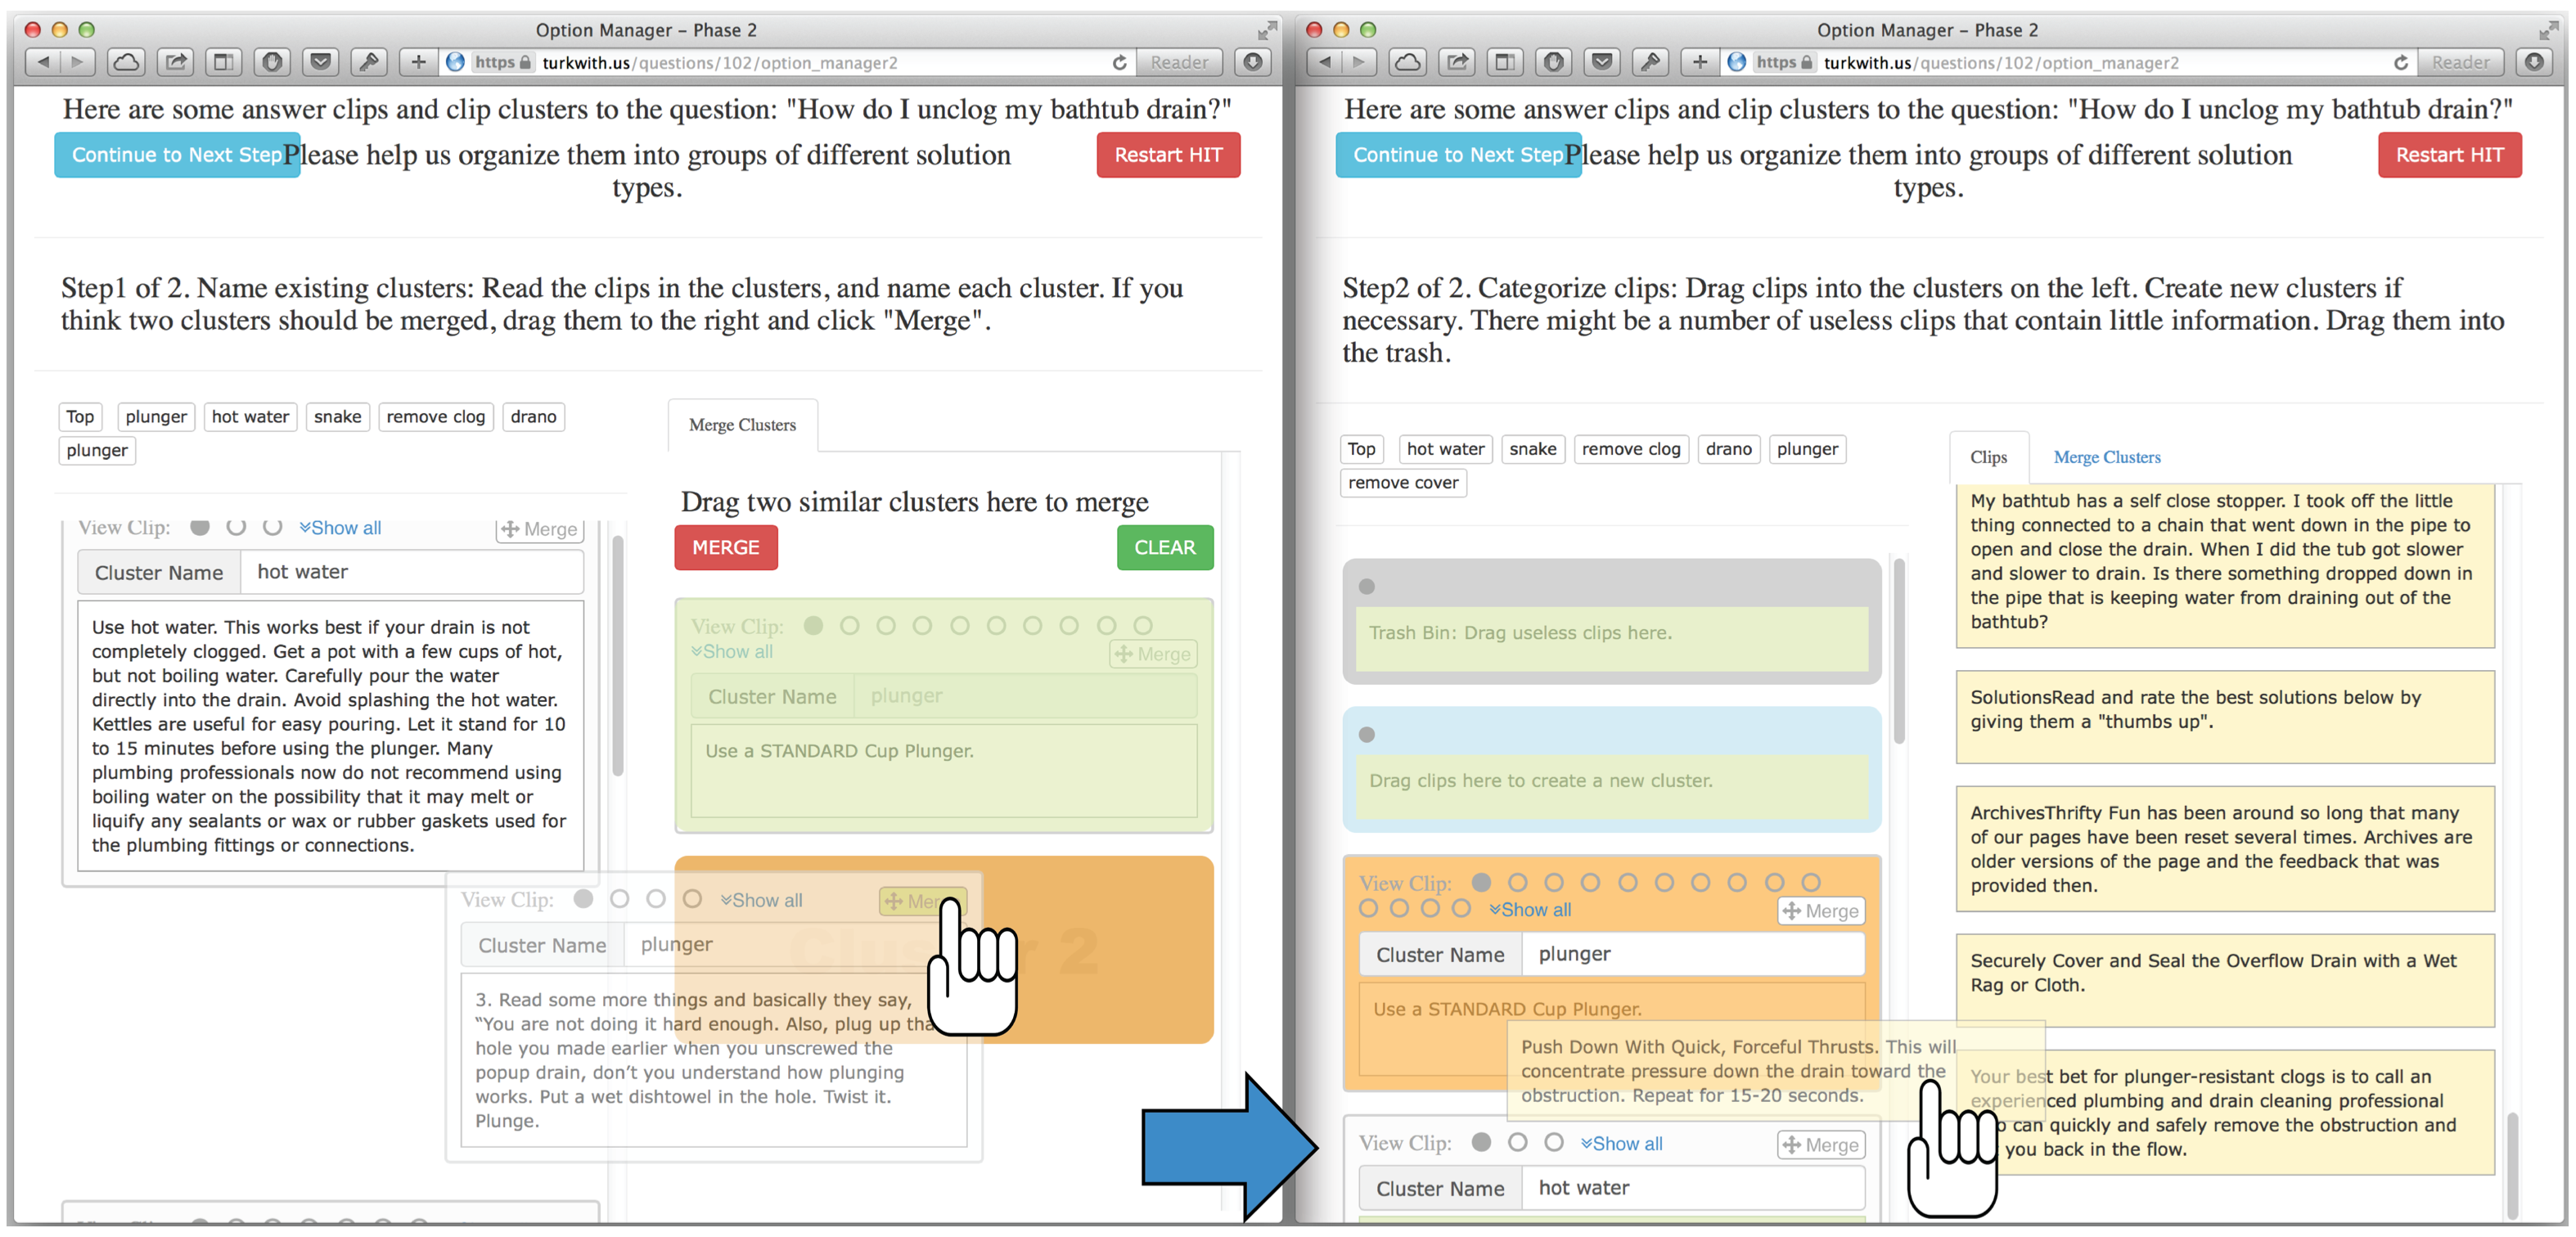
\includegraphics[width=2.1\columnwidth]{images/raw-01.png}
	\caption{The two steps HIT for Phase B: 1. Naming and merging existing
		clusters and 2. Clustering remaining clips.}
	\label{fig:phase2-hit}
\end{figure*}


\subsection{Phase B: Global Clustering}

Once the set of clusters and unclustered clips is obtained from Phase A, they
are presented to new crowdworkers with the instruction to cluster the remaining
clips in the following two stages of Phase B. The intuition behind this
is that even though machine learning techniques can produce high
performance output, sometimes it is achieved at the expense of sacrificing the
border cases. Human-guided ``clean up'' is often necessary for data produced by a
machine learning model.  

\subsubsection{Stage 1. Clustering with global constraint}

In the first stage of Phase B, we present the partially clustered dataset to
the crowdworkers.  As shown in Figure~\ref{fig:phase2-hit}, the process consists
of two steps:

\begin{enumerate}
	\item We present the clusters generated from Phase A on the
		left of the screen, and crowdworkers are instructed to review and name
		each cluster.  This process helps the workers build up a global
		understanding of the dataset and the abstraction level of the
		existing clusters. At this point, they can also merge existing
		clusters by dragging two clusters into the placeholders on the right.
		This allows the workers to further organize the existing clusters into
		coherent classes by merging duplicate or similar clusters that may
		have been created based on synonymous keywords in Phase A (e.g., \emph{hot
			water} and \emph{boiling water}).
	\item After naming existing clusters, the crowdworkers are then
		instructed to cluster the remaining clips shown on the right. In this
		process, the workers can: 1. Drag clips into existing clusters, 2.
		Create new clusters by dragging a clip over the blue placeholder, or;
		3.  Remove uninformative clips by dragging them into the trash
		bin.
\end{enumerate}

\subsubsection{Stage 2. Integrate clusters from multiple crowdworkers}

In the second and final stage, we use the hierarchical clustering method again
to aggregate and combine different solutions from the crowdworkers into a final
result. This time, we use a different similarity measure between two clips
based on the number of crowdworkers who assigned them in the same cluster:


\begin{equation}
	ClipSim(t_1, t_2) = \frac{1}{N} |\{\omega_j \forall t_1, t_2 \in \omega_j \; and \; \omega_j \in \Omega\}|
\end{equation}

where $t_1, t_2$ are the two clips, $N$ is the total number of crowdworkers,
$\Omega$ is the set of all clusters created by all crowdworkers. This
similarity function is robust against a few crowdworkers doing a
poor job. For example, if one crowdworker assigned every clip in the dataset to
a single, general cluster (e.g., \emph{answers}), the effect to the similarity function
would be equivalent to having one less crowdworker and applying Laplacian smoothing.

We use the similarity function with a threshold of 0.5 (voting majority) to
perform hierarchical clustering as described in the previous subsection to
produce the final output.


